\setlength{\footskip}{8mm}

\chapter{Literature Review} 
\label{ch:literature-review}

\textit{Some intro..}

\section{Software Architecture of Autonomous Driving Vehicle}
\label{section-name-in-literature-review}

\shortciteA{sbehere16t} has split the major components of the motion control part of the autonomous driving system into three main categories as shown in Figure \ref{fig:fav_automonous}. These categories are

\begin{itemize}
	\item Perception of the external environment in which the vehicle operates
	\item Decisions and control of the vehicle motion, with respect the external environment that is perceived
	\item Vehicle platform manipulation which deals mostly with sensing, control and actuation of the Ego vehicle, with the intention of achieving desired motion.
\end {itemize}

Each category can be further broken down into several components.

\subsection{Perception}

The \textbf{sensing components} senses the states of the vehicle and the states of the environment in which the vehicle operates. The \textbf{sensor fusion component} considers multiple sources of information to construct a hypothesis about the state of the environment. The \textbf{localization component} determines the location of the vehicle with respect to a global map. The \textbf{semantic understanding component} processes the sensor input and derives meaningful information form it. The \textbf{world model component} holds the state of the external environment.

\subsection{Decision and Control}
The \textbf{trajectory generation component} repeatedly generates a set of obstacle free trajectories in the world coordinate system and pick an optimal trajectory from the set.  \textbf{Energy management components} deals with energy management of the vehicle. \textbf{Diagnosis and fault management} monitors state of the overall system and its components. \textbf{Reactive control components} are used for immediate responses to unanticipated stimuli from the environment. The \textbf{vehicle platform abstraction component} refers to a minimal model of the vehicle platform. 

\subsection{Vehicle Platform Manipulation}

The \textbf{platform stabilization components}'s task is to keep the vehicle platform in a controllable state during operation. The \textbf{trajectory execution components} are responsible for executing the trajectory generated by Decision and Control. 

\begin{figure}
	\centering
	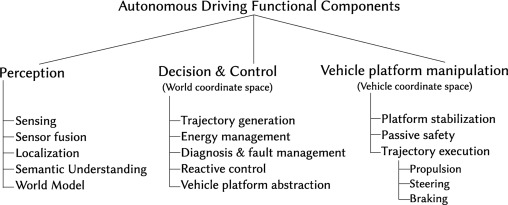
\includegraphics[width=5in]{figures/fav_autonomous_driving}
	\caption[FAV of Antonomous Driving System.]{\small 
		Functional Architecture View of Autonomous Driving System. Reprinted from work of \shortciteA{sbehere16t} }
	\label{fig:fav_automonous}
\end{figure}

\section{Coordinate Systems}
	
\subsection{Earth Centric, Earth Fixed}

The earth-centered earth-fixed (ECEF), rotates with the Earth and has its origin at the center of the Earth. Figure \ref{fig:coordinatesystem} a.

It follows the right hand coordinate system. And \shortcite{coordinatesystem} describes it as:

\begin{itemize}
	\item The origin at the center of mass of the Earth, a point close to the Earth's center of figure
	\item The Z axis on the line between the North and South Poles, with positive values increasing northward (but does not exactly coincide with the Earth's rotational axis)
	\item The X and Y axes in the plane of the Equator
	\item The X axis passing through extending from 180 degrees longitude at the Equator (negative) to 0 degrees longitude (prime meridian) at the Equator (positive)
	\item The Y axis passing through extending from 90 degrees west longitude at the Equator (negative) to 90 degrees east longitude at the Equator (positive)
\end{itemize}

\subsection{Local tangent plane}

In local tangent coordinate system, a position in earth is fixed as the origin. There are two conventions as shown in Figure \ref{fig:coordinatesystem} b.

\begin{itemize}
	\item East(x), North(y), UP(z) (ENU).
	\item North(x), East(y), Down(z) (NED), which is mostly used is aviation as the objects of interest lies before an aircraft.
\end{itemize}

\begin{figure}%
	\centering
	\subfloat[\small Earth Centric, Earth Fixed coordinate system. By Krishnavedala - Own work, CC BY-SA 3.0]{{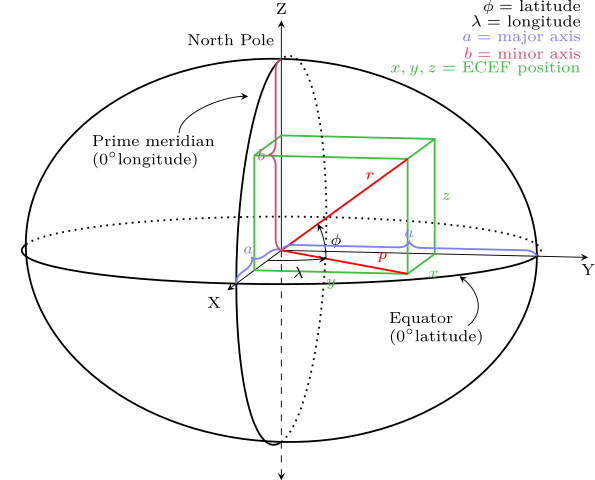
\includegraphics[width=3in]{figures/ECEF}}}%
	\subfloat[\small Local tangent plane coordinate systems]{{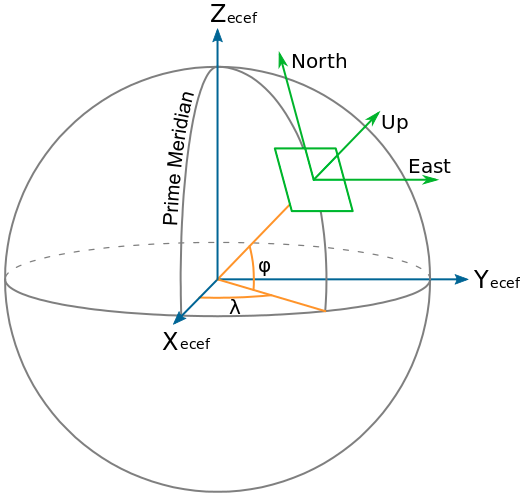
\includegraphics[width=3in]{figures/ENU_NED}}}%
	\caption[ECEF coordinate system]{\small Coordinate Systems
	}%
	\label{fig:coordinatesystem}%
\end{figure}

\subsection{Pixhawk and ROS coordinates}

Pixhawk follows NED convention, whereas ROS follows ENU convention. The conversion between these different conventions is handled automatically by MAVROS. For translate airframe related data rotation of 180° is applied about ROLL (X) axis. For local 180° rotation is applied about ROLL (X) and 90° about YAW (Z) axes.

ROS has other reference frames as described in \shortcite{rosrefframes}.

\begin{itemize}
	\item The coordinate frame called \textbf{base\_link} is rigidly attached to the mobile robot base. It can be attached in any arbitrary position or orientation.
	\item The coordinate frame called \textbf{odom} is a world-fixed frame. The pose of a robot is continuous in this frame, but it can drift over time.
	\item The coordinate frame called \textbf{map} is a world fixed frame, with its Z-axis pointing upwards. 
	\item The coordinate frame called \textbf{earth} is the origin of ECEF.
\end{itemize}

The relationship between these frames is shown in Figure \ref{fig:rosrefframes}.

\begin{figure}
	\centering
	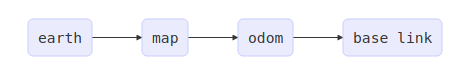
\includegraphics[width=5in]{figures/ros_rel_frames}
	\caption[FAV of Antonomous Driving System.]{\small 
	Relationship between ros frame. \shortciteA{rosrefframes} }
	\label{fig:rosrefframes}
\end{figure}

\section{Simultanious Localization and Mapping}

\shortcite{slamp1} describes SLAM problem as a process by which a mobile robot can build a map of an environment and at the same time use this map to deduce its location. In SLAM, both the trajectory of the platform and the location of all landmarks are estimated online without the need for any a priori knowledge of location.

In probabilistic SLAM, the probability distribution, 
\begin{equation} \label{eq:slam1}
P({\bf x}_{k},{\bf m}\vert {\bf Z}_{0:k},{\bf U}_{0:k},{\bf x}_{0})
\end{equation}
has to be computed at any time instance $k$. Where
\begin{itemize}
	\item ${\bf x}_k$: the state vector describing the pose of the vehicle.
	
	\item ${\bf u}_k$: the control vector, applied at time $k - 1$ to drive the vehicle to a state ${\bf x}_k$ at time $k$.
	
	\item ${\bf m}_i$: a vector describing the location of the $ith$ landmark whose true location is assumed time invariant. This is the map of the environment.
	
	\item ${\bf z}_{ik}$: an observation taken from the vehicle of the location of the $ith$ landmark at time $k$.
	
	\item ${\bf m}$: the set of all landmarks detected
	
	\item ${\bf Z}_{0:k}$: the set of all observations upto time $k$
	
	\item ${\bf U}_{0:k}$: the set of all control input upto time $k$
	
\end{itemize}

The best estimate of ${\bf x}_k$ (pose) and ${\bf m}$ (map) at any time instance $k$ would be maximizing \ref{eq:slam1}.

The \textit{observation model} describes the probability of making an observation ${\bf z}_k$ when the vehicle location and landmark locations are known and is generally described in the form
\begin{equation}
P({\bf z}_{k}\vert {\bf x}_{k},{\bf m})
\end{equation}

The\textit{ motion model} for the vehicle can be described in terms of a probability distribution on state transitions in the form
\begin{equation}
P({\bf x}_{k}\vert {\bf x}_{k-1},{\bf u}_{k})
\end{equation}

The state transition is assumed to be a Markov process which is independent of both the observations and the map. The next state ${\bf x}_k$ depends only on the immediately preceding state ${\bf x}_{k−1}$ and the applied control ${\bf u}_k$.

Now, the pose of the vehicle and map can be estimated by standard two-step recursive (sequential) prediction (time-update) correction (measurement-update) form:

\textbf{Time Update}
\begin{equation}
P({\bf x}_{k},{\bf m}\vert {\bf Z}_{0:k-1},{\bf U}_{0:k},{\bf x}_{0})= \int P({\bf x}_{k}\vert {\bf x}_{k-1},{\bf u}_{k}) \quad\times P({\bf x}_{k-1},{\bf m}\vert {\bf Z}_{0:k-1}, {\bf U}_{0:k-1},{\bf x}_{0}){\rm d}{\bf x}_{k-1}
\end{equation}

\textbf{Measurement Update}
\begin{equation}
P({\bf x}_{k},{\bf m}\vert {\bf Z}_{0:k},{\bf U}_{0:k},{\bf x}_{0}) = {P({\bf z}_{k}\vert {\bf x}_{k},{\bf m})P({\bf x}_{k}, {\bf m}\vert {\bf Z}_{0:k-1},{\bf U}_{0:k},{\bf x}_{0})\over P({\bf z}_{k}\vert {\bf Z}_{0:k-1},{\bf U}_{0:k})}
\end{equation}

An alternate way of formulating the problem would be.

If the location of the vehicle ${\bf x}_k$ is know at all times. The map can be estimated by computing
\begin{equation}
P({\bf m}\vert {\bf X}_{0:k},{\bf Z}_{0:k}, {\bf U}_{0:k})
\end{equation}
. 

If the landmark locations are known, the vehicles can be localized by computing
\begin{equation}
P({\bf x}_k\vert {\bf Z}_{0:k},{\bf U}_{0:k}, m)
\end{equation}

\section{Visual SLAM}
Visual SLAM use images from one or more cameras for observation of the landmarks. \shortciteA{taketomi2017} has done a survey of Visual SLAM algorithm from 2010 to 2016. Visual SLAM can be categorized into feature based and direct methods. Feature based methods extract features from the input image and use those features as observations.

Feature based vSLAM cannot perform well in environments which is feature-less or texture-less. Further-more the point clouds produced by feature based methods is sparse. Some of the feature based vSLAM algorithms are:

\begin{itemize}
	\item Parallel Tracking and Mapping (PTAM) \cite{4538852}
	\item ORB SLAM \cite{7219438}
	\item ORB SLAM2 \cite{7946260}
	
\end{itemize}


Direct vSLAM takes the whole image for tracking and mapping and produces dense point clouds. Some of the feature less vSLAM algorithms are:

\begin{itemize}
	\item Dense Tracking and Mapping (DTAM) \cite{6126513}
	\item Large-Scale Direct SLAM (LSD SLAM) \cite{Engel2014LSDSLAMLD}
\end{itemize}

vSLAM algorithms have three basic modules 
\begin{enumerate}
	\item Initialization: Global coordinate system is defined, and the initial map is constructed from the environment.
	\item Tracking: The reconstructed map is tracked to estimate the pose of the camera in the global coordinate system.
	\item Mapping: Map is expanded if the camera observes unknown regions.
\end{enumerate}

Other modules that is used to increase stability and accuracy of vSLAM are:
\begin{enumerate}
	\item Re-localization: If tracking is lost, re-localization helps is recovering the camera pose in the global coordinate system.
	\item Global map optimization: The reconstructed map accumulates estimation error over distance the camera is moved. This module minimizes the error. Loop closing can estimate the accumulated error, if a region that has been observed is encountered again. Bundle adjustment optimizes the map and the camera poses to minimize the accumulated error.
\end{enumerate}


The limitation of vSLAM algorithms which can hinder its usage in practical applications as mentioned by \shortciteA {taketomi2017} are

\begin{itemize}
	\item Purely rotational movement: Monocular vSLAM cannot continue mapping when purely rotational movement is applied as disparities cannot be observered.
	\item Map initialization: To get an accurate initial map, the distance between two images should be large while tracking the same features. 
	\item Estimating Intrinsic camera parameters: The cameras to be used has to be calibrated beforehand, and the  camera matrix $K$ and the distortion coefficients $d1, d2, p1, p2$ has to be known.
	\item Rolling shutter distortion:Cheap camera has a rolling shutter which may and the same image may has different sections taken from different camera pose.
	\item Scale Ambugity: In monocular vSLAM, absolution scale is unknown. Hence the pose and map generated may not be on scale with the actual world coordinates.
\end{itemize}




\subsection{ORB SLAM}

ORB SLAM \cite{7219438} is a monocular feature based vSLAM algorithm. It uses ORB feature detectors and the same features are used in mapping as well as tracking. It has three threads running in parallel for tracking, local mapping, and loop closing as shown in Figure \ref{fig:orb_slam1}.

\textbf{Automatic Map Initialization} is done by finding corresponding ORB features in initial frames $F_c$ and reference frame $F_r$. Then in parallel thread, homography ${\bf H}_{cr}$ and fundamental ${\bf F}_{cr}$ matrix are calculated. At each iteration a score $S_M$ is computed. Then homography and fundamental matrix with the highest score is chosen. If there are no candidate models, the process is repeated again. For a planar scene homography is chosen, or else fundamental matrix. In case of homography eight motion hypothesis is retrieved. The solution with most points seen in parallax in front of both the camera with low re-projection error is chosen. In the case of the fundamental matrix, it is converted into an essential matrix using the calibration matrix $K$ as and four motion hypothesis are derived. The the possible solution is chosen in the same way as in homography. Then bundle adjustment is done to refine the initial construction.

In \textbf{tracking} images are divided into cells, and atleast 5 features per cell is extracted using ORB descriptor. If some cells do not have any corners, then the features per cell is adapted. If tracking was successful for last frame, a constant velocity motion model is used to predict the camera pose and perform a guided search of the map points observed in the last frame. If the motion model is violated, a wider search is performed of the map points around their position in the last frame. The pose is then optimized with the found correspondences. If the tracking is lost, the frame into bag of words and query the recognition database for keyframe candidates for global relocalization. After getting estimation of the camera pose and an initial set of feature matches, the map is projected into the frame and more map point correspondences are searched. The camera pose is optimized with all the map points found in the frame. Then the decision to add the current frame as a new keyframe is taken. To insert a new keyframe, more than 20 frames must have passed from the last global relocalization, local mapping is idle, or more than 20 frames have passed from last keyframe insertion, current frame tracks at least 50 points and less than 90\% points than reference keyframe.

In \textbf{local mapping} every new keyframe $K_i$ is analysed. The covsibility graph is updated with $K_i$.The spanning tree linking $K_i$ with the keyframe with most points in common is updated along with computing the bags of words representation of the keyframe, which will help in the data association for triangulating new points.Recent Map Points Culling is done to so that only few outliers are present.New map points are created by triangulating ORB from connected keyframes in the covisibility graph. Positive depth in both cameras, parallax, reprojection error, and scale consistency is checked. Local Bundle Adjustment is done to optimize the currently processed keyframe, all the keyframes connected to it in the covisibility graph, and all the map points seen by those keyframes. Outliers are discarded at during the optimization. Local Keyframe Culling detects redundant keyframes and delete them.

In \textbf{loop closing}  the last keyframe processed by local mapping is taken and tries to detect and close loops.Loop Candidates Detection is done by taking the bag of words vector of the current keyframe and comparing the similarity with its neighbour and keeping the least score. Then all the keyframe which has lower score is removed from the recognition database. All those keyframes directly connected to current keyframe is removed. Similarity Transformation is calculated between the current frame and the loop candidate. If the similarity is supported by enough inliers, then the loop with current keyframe is accepted. Loop correction is done to fuse duplicated map points and insert new edges in the covisibility graph that will attach the loop closure.Then pose graph optimization over the essential graph is done that distributes loop closing error along the graph. 


\begin{figure}
	\centering
	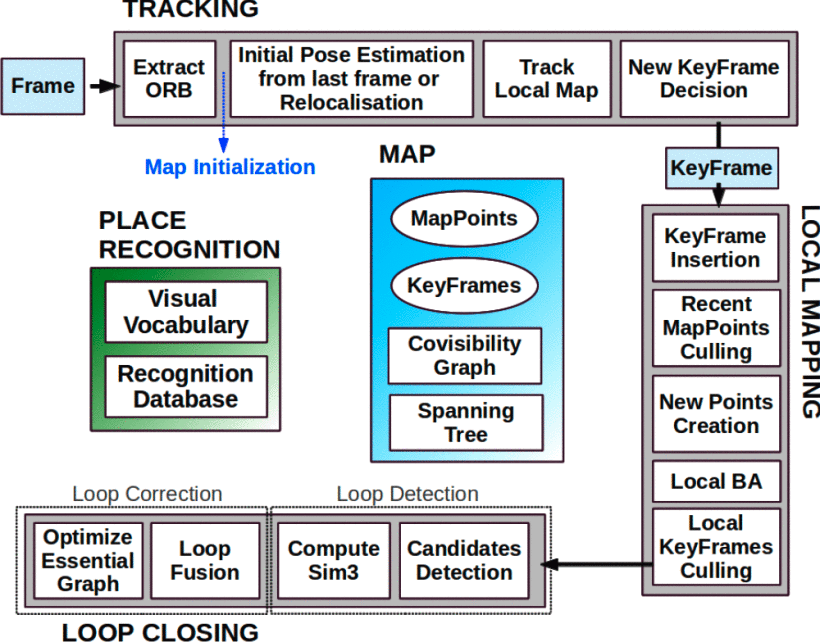
\includegraphics[width=5in]{figures/orb_slam1}
	\caption[ORB SLAM architecture]{\small 
		ORB SLAM system overview. Reprinted from work of \shortcite{7219438} }
	\label{fig:orb_slam1}
\end{figure}

\subsection{Visual Inertial ORB SLAM}

Visual Inertial ORB SLAM \shortcite{DBLP:journals/corr/Mur-ArtalT16} extends upon ORB SLAM by integrating stream of IMU measurement which solves the scale ambiguity problem of monocular SLAM.

IMU's reference frame is considered as ${\bf B}$. Camera and IMU are considered rigidly attached and the transformation ${\bf T}_{CB}$ which can be obtained through calibration.

\begin{equation}
{\bf T}_{CB} = [{\bf R}_{CB} \vert _C{\bf p}_B]
\end{equation}

The IMU orientation ${\bf R}_{WB}$, position $_W{\bf p}_B$ and velocity $_W{\bf V}_B$ in world reference frame $W$ can be computed as

\begin{align} \mathbf {R}^{k+1}_\mathtt {WB} = & \mathbf {R}^{k}_\mathtt {WB} \, \text{Exp}\left(\left(\boldsymbol {\omega }^k_\mathtt {B} - \boldsymbol {b}^k_g\right)\Delta t\right) \nonumber\\ _\mathtt {W}\mathbf {v}^{k+1}_\mathtt {B} = & {_\mathtt {W}\mathbf {v}^{k}_\mathtt {B}} + \mathbf {g}_\mathtt {W} \Delta t + \mathbf {R}^{k}_\mathtt {WB} \left(\boldsymbol {a}^k_\mathtt {B} - \boldsymbol {b}^k_a\right)\Delta t \nonumber\\ _\mathtt {W}\mathbf {p}^{k+1}_\mathtt {B} = & {_\mathtt {W}\mathbf {p}^{k}_\mathtt {B}} + {_\mathtt {W}\mathbf {v}^{k}_\mathtt {B}} \Delta t + \frac{1}{2}\mathbf {g}_\mathtt {W} \Delta t^2 + \frac{1}{2} \mathbf {R}^{k}_\mathtt {WB} \left(\boldsymbol {a}^k_\mathtt {B} - \boldsymbol {b}^k_a\right)\Delta t^2 \end{align}

Where
\begin{itemize}
	\item ${\omega }_{B}$ is the angular velocity of IMU.
	\item ${a}_{B}$ is the acceleration of the IMU
	\item $b_a$ and $b_g$ are the slowly varying bias of the accelerometer and gyroscope
	\item $g_w$ is the acceleration due to gravity
\end{itemize}

Using IMU preintegration, 

\begin{align} \label{eq:imuslam1} \mathbf {R}^{i+1}_\mathtt {WB} = & \mathbf {R}^{i}_\mathtt {WB} \Delta \mathbf {R}_{i,i+1} \text{Exp}\left(\left(\mathbf {J}^g_{\Delta R}\mathbf {b}^i_g\right)\right) \nonumber\\ _\mathtt {W}\mathbf {v}^{i+1}_\mathtt {B} = & {_\mathtt {W}\mathbf {v}^{i}_\mathtt {B}} + \mathbf {g}_\mathtt {W} \Delta t_{i,i+1} \nonumber\\ &+ \mathbf {R}^{i}_\mathtt {WB} \left(\Delta \mathbf {v}_{i,i+1} + \mathbf {J}^g_{\Delta v} \mathbf {b}^i_g + \mathbf {J}^a_{\Delta v} \mathbf {b}^i_a\right) \nonumber\\ _\mathtt {W}\mathbf {p}^{i+1}_\mathtt {B} = & {_\mathtt {W}\mathbf {p}^{i}_\mathtt {B}} + {_\mathtt {W}\mathbf {v}^{i}_\mathtt {B}} \Delta t_{i,i+1} + \frac{1}{2}\mathbf {g}_\mathtt {W} \Delta t^2_{i,i+1} \nonumber\\ & + \mathbf {R}^{i}_\mathtt {WB} \left(\Delta \mathbf {p}_{i,i+1} + \mathbf {J}^g_{\Delta p} \mathbf {b}^i_g + \mathbf {J}^a_{\Delta p} \mathbf {b}^i_a\right) \end{align}

Preintegrations and Jacobians can be efficiently computed iteratively as IMU measurements arrive using \ref{eq:imuslam1}.

Hence we can localize the IMU using the stream of IMU measurement.

In \textbf{tracking}, the IMU pose is estimated and the camera pose is predicted. The keypoint in the camera frame is matched with projected map points. Optimization id done on current frame by minimizing the feature reprojection error of all matched points and an IMU error term. 

In \textbf{local mapping}, the keyframe N+1 is always included in the fixed window as it constrains the IMU states.The cost function is a combination of IMU error terms (6) and reprojection error terms. The local window in Visual-Inertial ORB-SLAM is retrieved by temporal order of keyframes, while in ORB-SLAM is retrieved using the covisibility graph.

In \textbf{loop closing} the pose-graph optimization is performed on 6 Degrees of Freedom(DoF) instead of 7 DoF [23], as scale is observable.  IMU model velocities are corrected by rotating them according to the corrected orientation of the associated keyframe.  BA in a parallel thread is done that optimizes all states, including velocities and biases. 

The \textbf{IMU initialization} has the following steps


In \textbf{gyroscope bias estimation} can be done from the known orientation of two consecutive keyframes. A constant bias $b_g$ is optimized which minimizes the difference between gyroscope integration and relative orientation computed from ORB-SLAM, for all pairs of consecutive keyframes.

In \textbf{scale and gravity approximation}, a scale  factor $s$ is computed which is used when transforming between camera $𝙲$ and IMU $𝙱$ coordinate systems.

In \textbf{accelerometer bias estimation, and scale and gravity direction refinement}, we include the gravity magnitute $G$ and the accelerometer bias.

In \textbf{velocity estimation}, three consecutive keyframes are taken into consideration when calculating the velocity of the most recent keyframe.

In \textbf{bias reinitialization after relocalization}, after the system relocalizes, gyroscope and accelerometer biases are re-estimated using 20 consecutive frames localized with only vision.



\FloatBarrier

